\documentclass{beamer}

% to include graphics
\usepackage{graphicx}

% to include hyperlinks
\usepackage{hyperref}

% divide slides into columns
\usepackage{multicol}


\usetheme{Copenhagen}
\usecolortheme{beaver}

\title{Cluster Progress}
\date{\today}

\begin{document}

%----------BEGIN TITLE----------

\begin{frame}
  \maketitle
\end{frame}

%-----------END TITLE-----------

%----------BEGIN NAS-0----------

\begin{frame}

  \frametitle{NAS-0 Drive Failures}

  \begin{itemize}
    \item There have been 3 drive failures in NAS-0.
    \item The spares have been used to replace two of the failures.
    \item One failed drive remains in the array.
    \item New 750GB drives have been ordered!
  \end{itemize}

  \begin{figure}[H]
    \begin{center}
      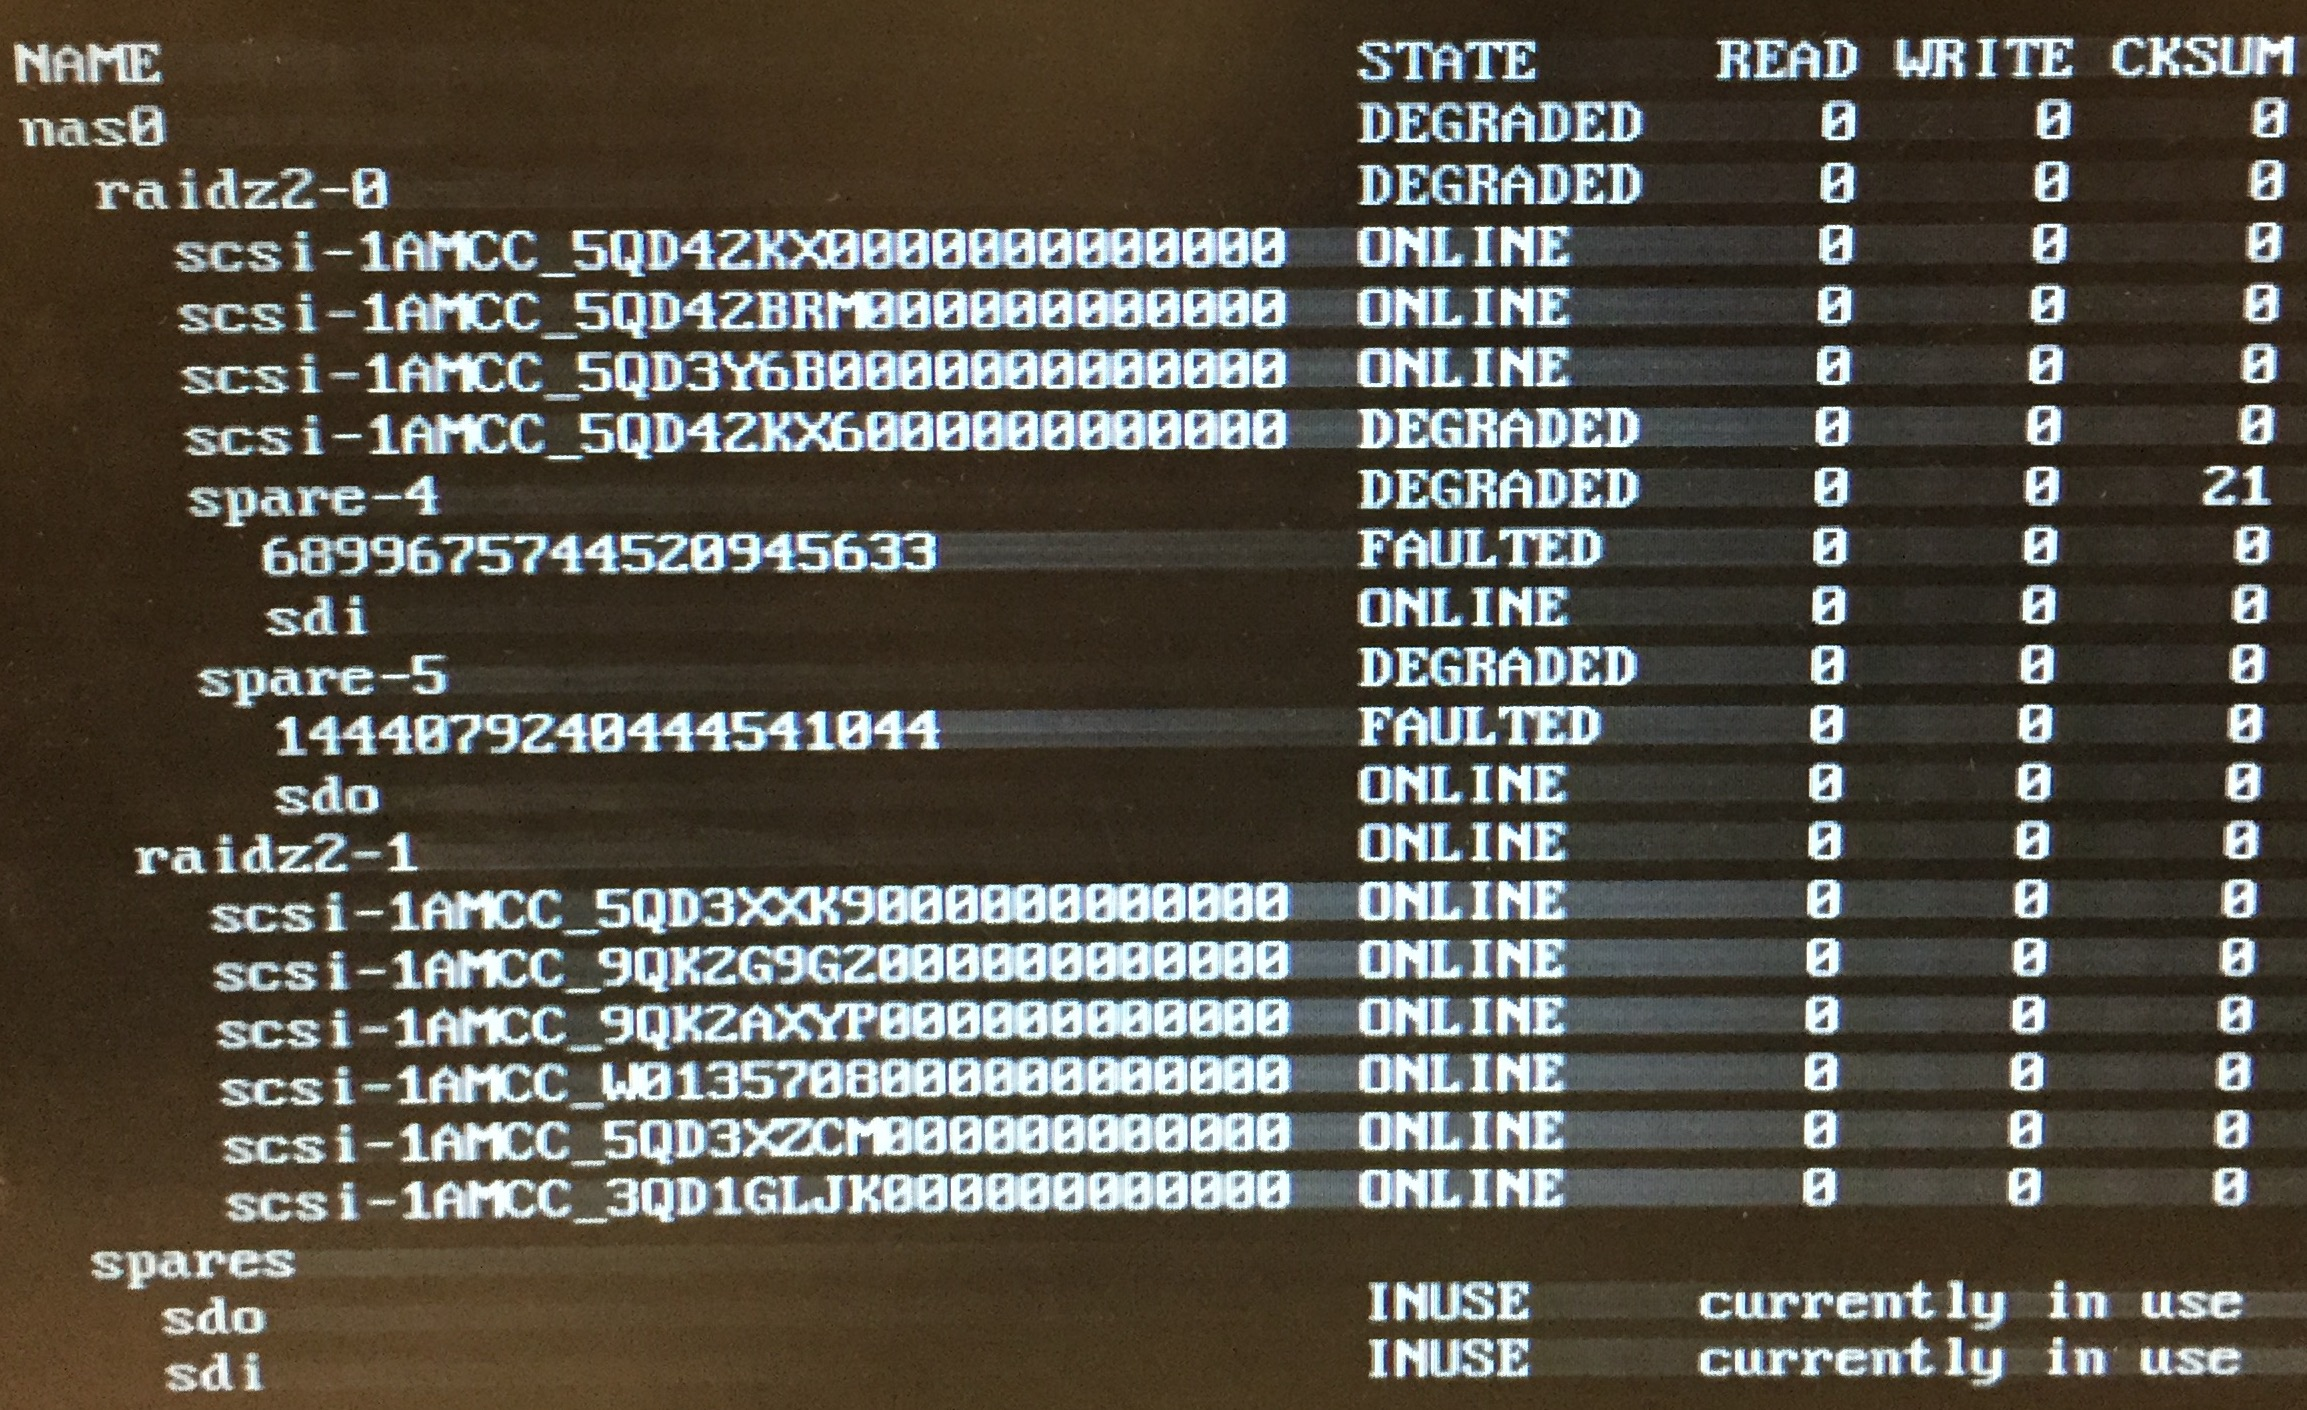
\includegraphics[width=0.7\textwidth]{nas0status.JPG}
    \end{center}
  \end{figure}

\end{frame}

%-----------END NAS-0-----------

%----------BEGIN OSG SOFTWARE SETUP----------

\begin{frame}

  \frametitle{Software Configuration}

    \textbf{HTCondor Testing:}
    
    \begin{itemize}
    \item We created and submitted a sample job.
    \item It didn't work.
    \end{itemize}  

    % screenshot of failed job

    \textbf{Preparing SE Software:}

    \begin{center}
      \begin{tabular}{|l|l|}
        \hline
        HDFS & filesystem for the SE's data drive \\
        PhEDEx & for transferring data from remote sources \\
        Squid & for easing data transfer \\
        XRootD & for data management \\
        \hline
      \end{tabular}
    \end{center}

\end{frame}

%-----------END OSG SOFTWARE SETUP-----------

\end{document}
